\section{Verwandte Arbeiten}

Um verwandte Arbeiten zu identifizieren wurde eine Literaturrecherche in der wissenschaftlichen Datenbank Google Scholar durchgeführt. \\
Dabei wurden die Keywords \glqq visual analysis\grqq, \glqq visualization\grqq , "\glqq offerings\grqq , \glqq used car\grqq  und \glqq online platform\grqq  verwendet und verschiedene wissenschaftliche Publikationen identifiziert. Zwei dieser Treffer sollen hier exemplarisch vorgestellt und Unterschiede und Gemeinsamkeiten der hier präsentierten Lösung identifiziert werden. \\

Das Forschungspapier \glqq  How much is my car worth? A methodology for predicting used cars prices using Random Forest \grqq \cite{pal2017much} präsentiert eine Methode zur Vorhersage von Gebrauchtwagenpreisen mithilfe von Random Forest. Die Autoren entwickeln ein Modell, das mithilfe von maschinellem Lernen den Preis von Gebrauchtwagen prognostiziert.\\
Für die Analyse des verwendeten Datensatzes, der von eBay-Kleinanzeigen stammt, nutzen die Autoren verschiedene Visualisierungen. Beispiele hierfür sind Bar-Charts, Boxplots und Scatterplots.  Einige der  Ergebnisse zeigen die Verteilung des Fahrzeugalters, den durchschnittlichen Preis nach Fahrzeugtyp, die Verteilung von Fahrzeugmarken und den Einfluss von reparierten Schäden auf den Fahrzeugpreis. \\

\begin{figure}[H]
    \centering
    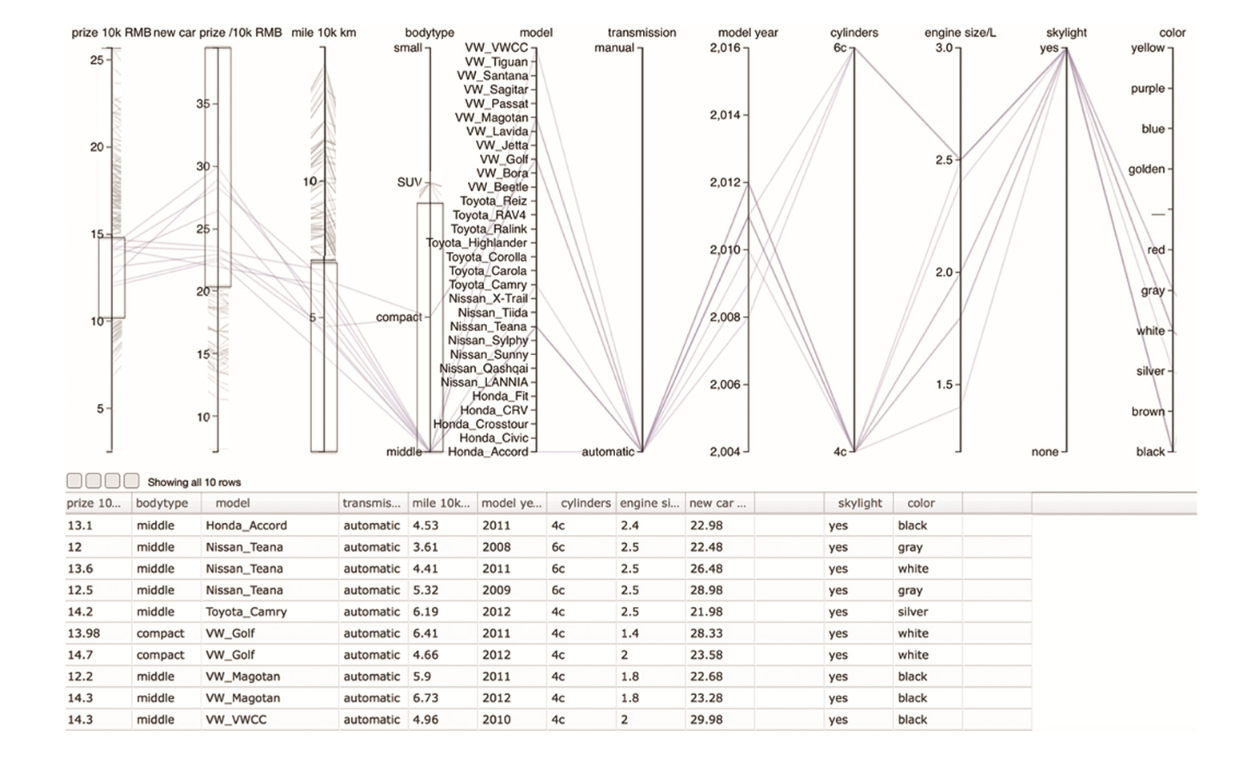
\includegraphics[width = \textwidth]{img/related_work.png}
    \caption{Vergleiche anderes Paper}
    \label{fig:related_work_vis}
\end{figure}

Die zweite Arbeit \cite{chen2017employing} beschäftigt sich mit der Verbesserung der Nutzerfahrung auf Gebrauchtwagen-Online-Plattformen mithilfe von Datenvisualisierungen. Die Autoren betonen die Komplexität der Daten und die Herausforderungen für Nutzer, zufriedenstellende Autos innerhalb ihres Budgets zu finden. \\

Sie analysieren das Verhalten von Autokäufern und entwickeln eine Datenvisualisierungsschnittstelle, wie sie auch im Kapitel zu Anwendungsfällen beschrieben ist. Die vorgestellte Parallelkoordinaten-Visualisierung ermöglicht es Benutzern, den Gebrauchtwagenmarkt zu verstehen, Beziehungen zwischen verschiedenen Attributen zu erkennen und Autos einfach zu suchen, filtern und vergleichen. Die Autoren identifizieren Probleme mit den aktuellen Suchmethoden, einschließlich Informationsüberlastung und -mangel, und stellen Designanforderungen vor. Die vorgeschlagene Schnittstelle ermöglicht es Benutzern, eine Übersicht des Marktes zu erhalten, Vorhersagen zu treffen, Kompromisse zwischen Attributen zu finden und eine geeignete Auswahl von Autos zu erstellen. Die Parallelkoordinaten-Plots werden auf der Suchseite implementiert, wobei verschiedene Parameter wie Preis, Typ, Kilometerstand, Baujahr und andere visuell dargestellt werden (Abbildung \ref{fig:related_work_vis}. Die Benutzer können mithilfe von Auswahlboxen auf den Achsen Suchbereiche festlegen und so eine engere Auswahl von Autos erstellen.\\
Insgesamt zeigt die Arbeit, wie Datenvisualisierung die Suche nach Gebrauchtwagen verbessern kann, indem sie dem Benutzer eine bessere Kontrolle, Vorhersagbarkeit und Verständnis des Marktes ermöglicht. \\

